%!TEX TS-program = xelatex
%!TEX root = ../../maxwell2018thesis.tex

\chapter[Operationalised Stopping Strategies]{Operationalised\\Stopping Strategies}\label{chap:strategies}
In Section~\ref{sec:stopping_background:heuristics}, we discussed a number of different \emph{stopping heuristics} that have been previously defined in the literature. In this chapter, we take a number of these stopping heuristics forward to produce a series of different \emph{stopping strategies,} providing an answer that addresses \darkblueboxbold{HL-RQ2}.\footnote{Refer to Section~\ref{sec:intro:rqs} on page~\pageref{sec:intro:rqs} for the definition of the research question.}

\begin{figure}[h]
    \centering
    \vspace{4mm}
    \resizebox{1\hsize}{!}{
    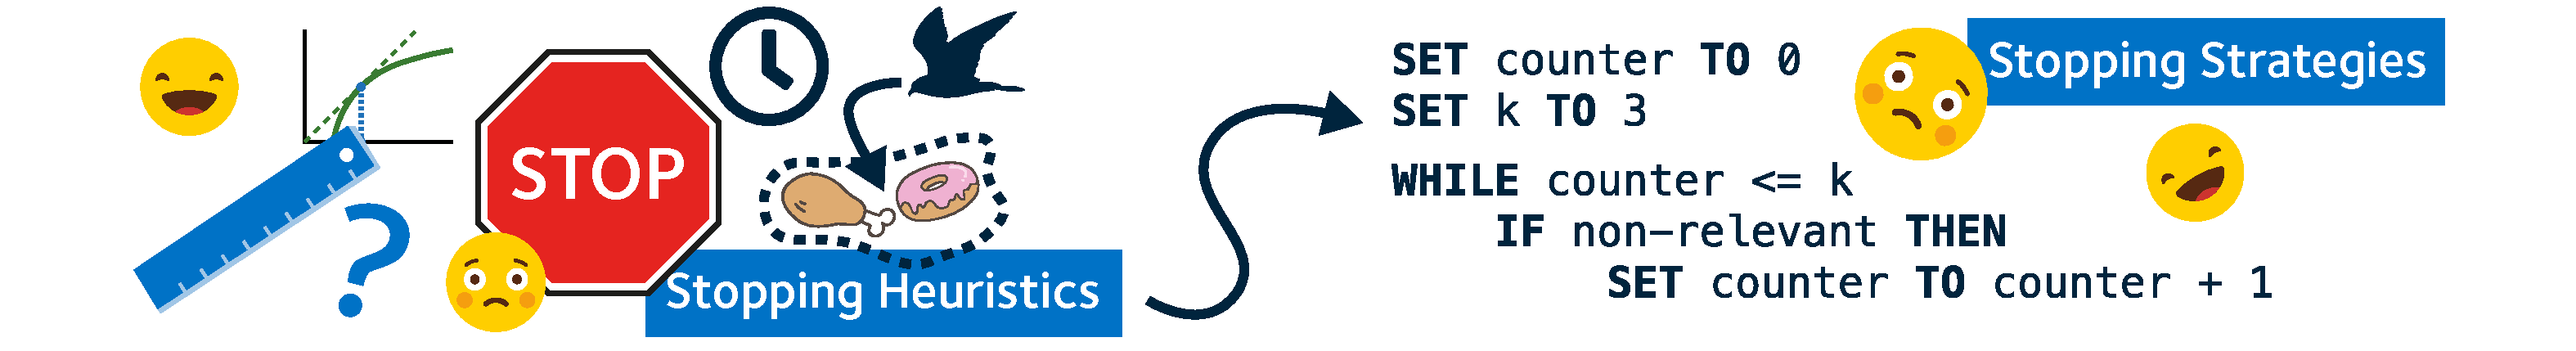
\includegraphics{figures/ch5-conversion.pdf}}
    \label{fig:conversion}
    \vspace{-5mm}
\end{figure}

These stopping strategies are operationalised versions of the corresponding heuristics. This means that we can subsequently implement and evaluate their effectiveness. We consider twelve different stopping strategies across seven different categories, the categories being:

\begin{itemize}
    \item{\blueboxbold{fixed depth}, which assumes a searcher examines to a fixed depth -- and is also considered to be our baseline approach;}
    \item{\blueboxbold{frustration}, considering a searcher's \emph{tolerance to non-relevance;}}
    \item{\blueboxbold{satisfaction}, taking into consideration how satisfied a searcher feels;}
    \item{\blueboxbold{difference}, which operationalises how \emph{different} new content appears to previously observed content;}
    \item{\blueboxbold{\gls{acr:ift}}, which considers a searcher's \emph{instantaneous intake;}}
    \item{\blueboxbold{time-based}, which utilise time as a measure for stopping; and}
    \item{\blueboxbold{measure-based}, considering an established~\gls{acr:ir} measure as a stopping strategy.}
\end{itemize}

In the remainder of this chapter, we consider each of the seven categories enumerated above. For each category, we discuss the different operationalised stopping strategies that we consider for the empirical work reported later in this thesis. Before this, we begin with a brief discussion about the different stopping decision points that were outlined in Section~\ref{sec:csm:stopping}, and the notation used hereon in when describing the different stopping strategies.

\blueboxheader{Considering Stopping Decision Points}
An open question is which of the different stopping strategies that we discuss in this chapter are applicable for the different \emph{stopping decision points,} as outlined in Section~\ref{sec:csm:stopping}. Indeed, the stopping strategies that we outline do not seem particularly applicable to the context of~\gls{acr:serp} level stopping, but could be applied to the session level stopping decision point. For example, the satisfaction/satiation based stopping heuristic would be particularly suited to a session that is goal-based in nature.

For the purposes of this thesis however, we consider the following stopping strategies purely in the context of \emph{result summary stopping,} or considering the depth to which a searcher will traverse a list of ranked results. These are examined in tandem with the new~\gls{acr:serp} level stopping decision point, and session-based stopping, where goal-based \emph{(find $x$ documents)} and time-based \emph{(stop after $y$ seconds have elapsed)} stopping heuristics are used. This will allow us to examine how the session goal directly influences the behaviours exhibited by searchers during the search session -- in particular, their stopping depths over each query.

\blueboxheader{A Note on Notation}
Each of the operationalised stopping strategies that are introduced in this chapter come complete with at least one \emph{stopping threshold} variable, allowing one to customise the point at which a searcher subscribing to a given stopping strategy should stop. As demonstrated in the \emph{Presentational Conventions} front matter, the notation we use to illustrate a stopping strategy and its threshold(s) is \dualbluebox{NAME}{THRESHOLD}. As an example, \dualbluebox{SS1-FIX}{@3} denotes the fixed depth stopping strategy \blueboxbold{SS1}, set to a threshold of $3$. This stopping strategy is outlined below in Section~\ref{sec:strategies:fixed}.

\section{Fixed Depth}\label{sec:strategies:fixed}
The fixed depth stopping strategy is based upon the assumption held across many of the models and measures widely used throughout the~\gls{acr:ir} community. The assumption is that a searcher, when examining a list of ranked results, searchers will browse to a \emph{fixed depth} before stopping. $P@k$, defined in Section~\ref{sec:ir_background:evaluation:system:precision}, is a prime example of this, and has been used in many different studies examining the simulation of interaction. Given then wide use of this fixed depth approach in historical and contemporary~\gls{acr:ir} and~\gls{acr:iir} research, we consider this stopping strategy as the baseline approach to which we will compare more advanced stopping strategies.

\begin{itemize}
    \item{\blueboxbold{SS1-FIX}} A searcher employing this stopping strategy will stop searching once they have observed $x_1$ result summaries (i.e. \dualbluebox{SS1-FIX}{x1}), regardless of the relevancy of each judged result summary.
\end{itemize}

\blueboxbold{SS1-FIX} is quite a na\"{i}ve stopping strategy as it assumes that all documents up to rank $x_1$ are considered attractive enough for a searcher to wish to consider in closer detail. On average, this strategy does make sense; on a per-query basis however, a searcher's behaviours may not make sense, and be a waste of the searcher's time.

\begin{figure}[t!]
    \centering
    \resizebox{1\hsize}{!}{
    
\includegraphics{figures/ch4-ss1.pdf}}
    \caption[Examples of the fixed depth stopping strategy, \blueboxbold{SS1}]{An example of the fixed depth stopping strategy, stylised in this thesis as \blueboxbold{SS1}. Here, a searcher has an information need for the conference \emph{CIKM 2015} in Melbourne, Australia. The left example shows the top five results for poor performing query, with few unattractive results (denoted by {
\includegraphics[height=\fontcharht\font`\d]{figures/ch0-cross.pdf}}); conversely, the right shows results for a query performing well, with many attractive results (denoted by {
\includegraphics[height=\fontcharht\font`\d]{figures/ch0-tick.pdf}}). With \dualbluebox{SS1}{@4}, the searcher will stop at a depth of \emph{4,} regardless of the perceived relevancy of the content provided.}
    \label{fig:ss1}
\end{figure}

For example, Figure~\ref{fig:ss1} demonstrates two~\glsplural{acr:serp} side by side. Given a searcher's desire to find pages providing information to \emph{CIKM 2015}\footnote{CIKM 2015 was a conference held in Melbourne, VIC, Australia in October 2015. The paper that initially presented many of the different stopping strategies outlined in this chapter was presented at said conference. Refer to~\cite{maxwell2015stopping_strategies}.}, two queries are issued. The query on the left yields poorer results than the query on the right, denoted by the 
\includegraphics[height=\fontcharht\font`\d]{figures/ch0-tick.pdf} and 
\includegraphics[height=\fontcharht\font`\d]{figures/ch0-cross.pdf} that denote relevant and non-relevant pages respectively. With \dualbluebox{SS1}{@4}, four result summaries are always examined before stopping, regardless of the perceived quality of the results. As a result, examining four documents for the query on the left is by and large a waste of the searcher's time -- a searcher would be better \emph{adapting} his or her behaviour depending upon the perceived quality of the ranked list.

\section{Frustration and Satisfaction}\label{sec:strategies:frus_disg}
We \blueboxbold{SS1} referred to as a \emph{fixed} stopping strategy, as it is not \emph{adaptive.} The remaining stopping strategies presented in this chapter are considered to be adaptive as the permit a searcher to adapt their stopping depth depending upon the result summaries that they observe in a ranked list. In this section, we propose three adaptive stopping strategies that are based upon a searcher's \emph{tolerance to non-relevance} and a simple \emph{goal-based} approach.

\subsection{Searcher Frustration}\label{sec:strategies:frus_disg:frustration}
We first discuss the operationalisation of the frustration stopping heuristics, as outlined in Section~\ref{sec:stopping_background:heuristics:frustration}. Given a set of result summaries presented on a~\gls{acr:serp}, how many unattractive summaries would a searcher be prepared to examine before coming frustrated with the~\gls{acr:serp}, and abandoning it? This stopping heuristic attempts to address this question. Indeed, as detailed in Section~\ref{sec:stopping_background:heuristics}, a number of researchers have proposed stopping heuristics that consider unattractiveness.

The frustration heuristic intuitively makes sense for exhaustive searchers~\citep{kraft1979stopping_rules}. As an example, when tasked to find as many documents as possible related to different species of animals that are endangered, becoming disgusted with the presented results when a lack of animal species are shown would be a suitable point at which to break and reformulate a new query, or abandon the search session altogether.

From the heuristics defined by~\cite{cooper1973retrieval_effectiveness_ii} and~\cite{kraft1979stopping_rules}, we propose two variants of the frustration and disgust heuristics, \blueboxbold{SS2-NT} and \blueboxbold{SS3-NC}.

\begin{itemize}
    \item{\stoppingstratboxsingular{SS2-NT (Non-relevant, Total)} Under this stopping strategy, the searcher will stop once they have observed $x_2$ unattractive result summaries.}
    
    \item{\stoppingstratboxsingular{SS3-NC (Non-relevant, Contiguous)} Similar to the stopping strategy defined above above, a searcher employing this stopping strategy will stop once they have observed $x_3$ unattractive result summaries \emph{in a row (contiguously)}.}
\end{itemize}

\begin{figure}[t!]
    \centering
    \resizebox{1\hsize}{!}{
    
\includegraphics{figures/ch4-ss23.pdf}}
    \caption[Examples of frustration rules \stoppingstratboxsingular{SS2-NT} and \stoppingstratboxsingular{SS3-NC}]{An example of the two frustration rules, \stoppingstratboxsingular{SS2-NT} (left) and \stoppingstratboxsingular{SS3-NC} (right), both using a parameter of 3 unhelpful result summaries, under the same query and results. Given that \stoppingstratboxsingular{SS2-NT} considers the total number of result summaries judged to be unhelpful, a searcher employing this stopping strategy would stop at rank \emph{5} in the example above. Considering a set of contiguous unhelpful summaries, a searcher using \stoppingstratboxsingular{SS3-NC} would stop at rank \emph{7.}}
    \label{fig:ss23}
\end{figure}

With the adaptability of this stopping strategy to the presented results, this inherently makes the stopping strategy more realistic~\citep{moffat2013users_versus_models}. Figure~\ref{fig:ss23} illustrates this adaption in action, with the same query and associated results. On the left of the figure is an illustration of when a searcher employing \blueboxbold{SS2-NT} would stop, and on the right, an example of \stoppingstratboxsingular{SS3}. We use \dualbluebox{SS2-NT}{@3} and \dualbluebox{SS3-NC}{@3}. Under \blueboxbold{SS2-NT}, a searcher would stop at rank 5, while a searcher would stop at rank 7 when employing \blueboxbold{SS3-NC}.

For both \blueboxbold{SS2-NT} and \blueboxbold{SS3-NC}, any document that has been previously examined during the same search session (returned in the ranked results of a prior query) will be included in the count of non-relevant items. This is opposed to ignoring previously observed items, which has been shown in prior work to offer poorer performance~\cite{maxwell2015stopping_strategies}.

\subsection{Goal/Satisfaction-Based}
Analogous to frustration and disgust are the satisfaction, satiation and number-based stopping heuristics~\citep{cooper1973retrieval_effectiveness_ii, simon1955satiation, gibb1958number_rule}. Rather than focus upon the frustration or disgust that a searcher might experiences when confronted with unattractive result summaries, satisfaction-based stopping heuristics -- explained in Section~\ref{sec:stopping_background:heuristics:frustration} -- consider a searcher encountering a number of \emph{attractive} result summaries before deciding to stop.

\begin{itemize}
    \item{\stoppingstratboxsingular{SS4-SAT} A searcher using this stopping strategy will stop examining content after encountering $x_4$ attractive result summaries.}
\end{itemize}

While we consider this stopping strategy in the context of result summary level stopping, such a stopping strategy may not be particularly useful when operationalised at this stopping decision point. Consider the scenario where a searcher issues a poor query, yielding next to no summaries deemed to be worthy of further examination. In this scenario, a searcher fully complying with \blueboxbold{SS4} may struggle to find enough documents to reach their goal. This will mean that the searcher wastes time examining poor results. Such a stopping strategy may be better suited to an overall search goal (i.e. a session level stopping strategy), or at the session level stopping decision point. As a means of potentially avoiding a searcher becoming \emph{`trapped'} in an examination of a fruitless set of results, we consider an additional stopping strategy.

\subsection{Combining Frustration and Satisfaction}
The next stopping strategy proposed considered a combination of both the frustration/disgust and satisfaction/satiation stopping heuristics. This was named the \emph{combination heuristic} by~\cite{kraft1979stopping_rules}. Employing this stopping strategy, a searcher would stop either when they became frustrated, or were satisfied with the number of attractive summaries that they had observed -- whichever of the two criteria were met first. As such, we can convert this into a fifth stopping strategy, defined below.

\begin{itemize}
    \item{\stoppingstratboxsingular{SS5-COMB} A searcher utilising this stopping strategy will employ both frustration/disgust and satisfaction/satiation stopping heuristics to determine when to stop, ceasing their search on the~\gls{acr:serp} for the first stopping heuristic whose criterion is met.}
\end{itemize}

While \blueboxbold{SS4} can be selected as the operationalised satisfaction/satiation component, one of either \blueboxbold{SS2} or \blueboxbold{SS3} can be selected for the frustration/disgust component of this fifth stopping strategy. We discuss this in our general methodology in Section~\ref{sec:method:simulation:grounding:stopping}.

\section{Difference Threshold}
The next set of stopping strategies are based upon the difference threshold heuristic, as outlined in Section~\ref{sec:stopping_background:heuristics:difference} on page~\pageref{sec:stopping_background:heuristics:difference}. To operationalise this stopping heuristic, we considered the difference between a given result summary's snippet text, and the snippet texts of previously examined result summaries. Here, the idea was that aa searcher examined result summaries on a~\gls{acr:serp}, result summaries may be encountered that are not \emph{sufficiently different} from what had already been observed.\footnote{This means that searchers wouldn't be learning anything new~\citep{nickles1995judgment}, and thus would be wasting their time.} When encountering a result summary that is not sufficiently different, a searcher subscribing to the different threshold heuristic will then decide to stop.

From this stopping heuristic, we devised two separate stopping strategies where the difference between snippet texts were computed in different ways. The first approach considered the \emph{term overlap difference.}

\begin{itemize}
    \item{\stoppingstratboxsingular{SS6-DT (Difference, Terms)} This stopping strategy compares the occurrences of terms in a given result summary's snippet text against all terms in previously examined result summary snippets. If $\frac{|s_{curr} \cup s_{prev}|}{|s_{curr}|} > x_6$, the new snippet is then considered as too similar to previously examined result summaries. The searcher then abandons the present~\gls{acr:serp}.}
\end{itemize}

Essentially, \stoppingstratboxsingular{SS6-DT} considers that the more terms that overlap, the greater the chance that the new result summary does not contain any new information. In the definition above, $s_{curr}$ denotes the terms of the currently examined result summary snippet, $s_{prev}$ denotes terms from all previously observed result summary snippets, and $x_6$ is the threshold at which the searcher will stop.

The second difference based stopping strategy utilised~\gls{glos:kl}~\citep{kullback1951information} to determine how different a result summary is from those previously examined.

\begin{itemize}
    \item{\stoppingstratboxsingular{SS7-DKL (Difference, KL-Divergence)} This stopping strategy considers~\gls{glos:kl} as a means for comparing a given result summary snippet against those previously observed. If the resulting value is less than threshold $x_7$, the present result summary is considered to be too similar, and the searcher stops. The searcher then abandons the present~\gls{acr:serp}.}
\end{itemize}

Details related to the implementation of the difference heuristic stopping strategies can be found in Section~\ref{sec:method:simulation:grounding:stopping}.

\section{Instantaneous Intake}
In Section~\ref{sec:stopping_background:theoretical:ift:stopping}, we discussed several stopping heuristics that were derived from~\gls{acr:oft} and~\gls{acr:ift}. The~\gls{acr:ift}-based heuristic considers a searcher's \emph{optimal stopping point} at which a forager should stop, as suggested by the underlying models of~\gls{acr:ift}. This is calculated by observing a forager's \emph{average rate of gain.} If the value of what knowledge they gain drops below this threshold, the searcher should stop, as graphically illustrated in Figure~\ref{fig:ift_stopping} on page~\pageref{fig:ift_stopping}.

We now propose an eighth stopping strategy, this time based upon the notion of the average rate of gain accrued by a forager (or searcher).

\begin{itemize}
    \item{\stoppingstratboxsingular{SS8-IFT} With this stopping strategy, a searcher is assumed to have some idea of the average rate of gain (denoted as $x_8$). If the rate of gain from the observed documents thus far does not exceed $x_8$, the searcher then stops, and proceeds to undertake the next action as dictated by the~\gls{acr:csm}.}
\end{itemize}

Specific implementation details, such as how we computed the rate of gain, can be found in Section~\ref{sec:method:simulation:grounding:stopping}.

\section{Time-Based}\label{sec:strategies:time}
In addition to the optimal stopping point approach discussed above, Section~\ref{sec:stopping_background:theoretical:ift:stopping} also outlined a number of different~\gls{acr:oft}-inspired stopping heuristics that primarily used time as a measure of determining when to stop. From these approaches, we create two further time-based stopping strategies.

\begin{itemize}
    \item{\stoppingstratboxsingular{SS9-TIME} Based upon the \emph{time heuristic}~\citep{charles1972behaviour, krebs1973time_rule}, a simulated searcher using this stopping strategy will abandon a~\gls{acr:serp} after $x_9$ seconds have elapsed since they entered it.}
    
    \item{\stoppingstratboxsingular{SS10-RELTIME} Using the \emph{give-up heuristic}~\citep{krebs1974leave_after_rule}, a searcher will abandon a presented~\gls{acr:serp} $x_{10}$ seconds after the last document was considered relevant to the given information need.}
\end{itemize}

Given these stopping strategy definitions, \blueboxbold{SS9-TIME} performs akin to \blueboxbold{SS1-FIX}, in the sense it offers a fixed interaction time on each~\gls{acr:serp}, and is agnostic of the quality of the presented ranked list. Indeed, \blueboxbold{SS10-RELTIME} offers a more adaptive solution similar to \blueboxbold{SS2-NT} and \blueboxbold{SS3-NC}, basing the time at which the searcher stops $x_{10}$ seconds after a relevant document was last saved.

For this thesis, we also consider the \emph{combination heuristic} proposed by~\cite{mcnair1982gut_mvt}. The stopping strategy that we propose based upon this heuristic assumes that a searcher has been able to acquire an idea of how potentially relevant summaries \emph{distributed} across the results presented within the~\gls{acr:serp}.

\begin{itemize}
    \item{\stoppingstratboxsingular{SS11-COMB} When encountering a~\gls{acr:serp} expected to yield a high volume of relevant content early on (high scent), a searcher will employ the satisfaction/satiation stopping heuristic. If the~\gls{acr:serp} however yields relevant items over greater depths, or is judged to be of poor quality (low scent), the give-up heuristic is used instead.}
\end{itemize}

From our definitions above, \blueboxbold{SS4-SAT} is used for the satisfaction/satiation component, and \blueboxbold{SS10-RELTIME} is used for the give-up heuristic component. The combination stopping strategy attempts to ensure that a searcher does not waste time on a~\gls{acr:serp} that appear to offer a low yield, but conversely capitalise upon patches that present a high yield. Of course, determining the perceived yield is a question of implementation; refer to Section~\ref{sec:method:simulation:grounding:stopping} for more information on how we implemented this particular stopping strategy.

\section{Measure-Based}
The final proposed stopping strategy is based upon an established~\gls{acr:ir} measure.~\glsfirst{acr:rbp} -- as discussed in Section~\ref{sec:ir_background:evaluation:system:rbp} -- is utilised as the basis of our final stopping strategy. Under~\gls{acr:rbp}, the decision to continue to the next result in a ranked list is based upon a patience parameter, or the probability of continuing. Essentially,~\gls{acr:rbp} highlights that the probability of continuing decreases as a searcher progresses further down a ranked list.

\begin{itemize}
    
    \item{\stoppingstratboxsingular{SS12-RBP} With this stopping strategy, a searcher will stop examining a~\gls{acr:serp} when the likelihood of continuing falls below the~\gls{acr:rbp} probability computed at that rank, given a patience parameter $x_{12}$.}
    
\end{itemize}

By including such a measure, we provide a platform for which contemporary~\gls{acr:ir} measures can be compared against the performance of other stopping heuristics defined in the literature.

\section{Chapter Summary}
This chapter has outlined 12 different stopping strategies, all of which are based upon prior stopping heuristics and an established~\gls{acr:ir} measure. As such, this answer provides a possible answer to \darkblueboxbold{HL-RQ2}. In subsequent chapters of this thesis, we take these stopping strategies forward, discuss the specifics of how they were implemented in Section~\ref{sec:method:simulation:grounding:stopping}, and how they were employed in our empirical experimentation.